% Chapter 3

\chapter{Cut-minimal graphs and Cheeger graphs of a simplex}

\label{Chapter3}

In this chapter we start from the work of Kozlov (see \cite{1}) in which a graph theoretical approach to the first Cheeger constant of a simplex was developed. In the course of this approach the so called cut-minimal graphs appeared, which exactly describe \(1\)-cosystoles in a very intuitive way. As a consequence of the first main result of this chapter (Theorem \ref{theorem1}) we will determinine the dimension and partly the homology of the simplicial complex \(\mathcal{C}_1(\Delta^{[n]})\). In the second part of this chapter, we face the research on the first Cheeger constant of a simplex by investigating combinatorial properties of the Cheeger graphs which are just the graphic version of the \(1\)-Cheeger cosystoles. In particular, we show that \(h_1(\Delta^{[16]})>\frac{16}{3}\) holds, which strengthens our conjecture that \(h_1(\Delta^{[n]})>\frac{n}{3}\) holds in general for the case when \(n\) is a power of \(2\).

\section{Basic definitions and properties of cut-minimal graphs}
The following definition and some words about motivation and intuition for it can be found in \cite{1} (Definition 2.3).

\begin{defi}
Consider a graph \(G=([n],E)\). For any subsets \(A,B\subset [n]\) define
\[
E_G(A,B)\coloneqq \{(v,w)\in E\: :\: v\in A\text{, }w\in B\}
\]
and
\[
NE_G(A,B)\coloneqq \{(v,w)\notin E\: :\: v\in A\text{, }w\in B\}
\]
A graph \(G=([n],E)\) is called \textbf{cut-minimal}\index{Cut-minimal graph}, if for every \(S\subset[n]\) we have
\[
|E_G(S,[n]\setminus S)|\leq |NE_G(S,[n]\setminus S)|,
\]
which is equivalent to
\[
|E_G(S,[n]\setminus S)|\leq\frac{|S|(n-|S|)}{2}
\]
\end{defi}

Note, that there is a one-to-one correspondence between the graphs on \(n\) vertices and the \(1\)-chains  as follows:\\
For a graph \(G=([n],E)\) set \(c_G\coloneqq \sum\limits_{e\in E}e\in C_1(\Delta^{[n]})\) and for a chain \(c\in C_1(\Delta^{[n]})\) set \(G_c\coloneqq ([n],E)\), with \(E\coloneqq \supp(c)\). Considering characteristic cochains we also get a one-to-one corresponsing between graphs on \(n\) vertices and \(1\)-cochains and it is easy to see that a graph \(G=([n],E)\) is cut-minimal if and only if the corresponding cochain \(c_G^*\) is a cosystole.

\begin{rem}\label{remark1}
In fact for a graph \(G\) to be cut-minimal we only need to require the preceding condition holding for all \(S\subset [n]\), such that \(1\leq|S|\leq\frac{n}{2}\), since for all \(S\subset [n]\) we have \(E_G(S,[n]\setminus S)=E_G([n]\setminus S,S)\) and \(NE_G(S,[n]\setminus S)=NE_G([n]\setminus S,S)\).
\end{rem}

\begin{expl}
A simple cycle respresented by the graph \(G=([n],E)\) with\\
\(E\coloneqq \{(i,i+1)\: :\: 1\leq i\leq n-1\}\cup\{(n,1)\}\) is cut-minimal for all \(n\geq 7\) as follows. One can easily see that for all \(S\subset [n]\), such that \(|S|\leq\frac{n}{2}\), we have \(|E_G(S,[n]\setminus S)|\leq 2|S|\) and the inequality \(2|S|\leq\frac{|S|(n-|S|)}{2}\) holds for all \(n\geq |S|+4\), so by \(|S|\leq\frac{n}{2}\) the statement is true for all \(n\geq 7\).
\end{expl}

\begin{defi}
For any \(n\geq 3\) we define the set of all cut-minimal graphs on \(n\) vertices:
\[
CMG(n)\coloneqq \{G=([n],E)\: :\: G\text{ is cut-minimal}\}
\]
\end{defi}

Note, that for \(n\leq 2\) the set \(CMG(n)\) would be empty, so within this chapter we will always assume the number of vertices of cut-minimal graphs to be strictly larger than \(2\) without mentioning it again, since for the cases \(n\geq 2\) all statements we make are trivial.

\section{Maximal cut-minimal graphs}

Let us study the the topological and simplicial structure of the simplicial complex \(\mathcal{C}_1(\Delta^{[n]})\) which was, more generally, already introduced in the preceding chapter. Understanding this complex will help us to explore structural properties of the cut-minimal graphs on a certain number of vertices.\\
The first thing we will do is to determine the maximum number of edges, a cut-minimal graph on a certain number of vertices can have, which immediately gives us the dimension of \(\mathcal{C}_1(\Delta^{[n]})\).

\begin{prop}\label{proposition3}
\(C_{max}(\Delta^{[n]},1)\geq\binom{\left\lceil\frac{n}{2}\right\rceil}{2}+\binom{\left\lfloor\frac{n}{2}\right\rfloor}{2}\)
\begin{proof}
Let us construct a graph \(G\) on \(n\) vertices as follows. Choose a set \(V'\subset [n]\), such that \(|V'|=\left\lceil\frac{n}{2}\right\rceil\) and connect each pair of vertices from \(V'\) by an edge. Then connect each pair of the remaining \(\left\lfloor\frac{n}{2}\right\rfloor\) vertices by an edge. In other words our graph consists of two complete graphs. If \(n\) is even, they are identical, otherwise they differ by one vertex. In total we get \(\binom{\left\lceil\frac{n}{2}\right\rceil}{2}+\binom{\left\lfloor\frac{n}{2}\right\rfloor}{2}\) edges. We will show that this graph is cut-minimal.\\
Let \(S\subset [n]\) and define \(A\coloneqq S\cap V'\) and \(B\coloneqq S\setminus A\). If \(n\) is even, we have:
\begin{align}
|E_G(S,[n]\setminus S)|&=|A|(\frac{n}{2}-|A|)+|B|(\frac{n}{2}-|B|)\notag\\
&=\frac{n|A|}{2}-|A|^2+\frac{n|B|}{2}-|B|^2\notag\\
&=\frac{n|S|}{2}-(|A|^2+|B|^2)\notag
\end{align}
\begin{align}
&\leq\frac{n|S|}{2}-\frac{|S|^2}{2}\notag\\
&=\frac{|S|(n-|S|)}{2},\notag
\end{align}
where the inequality comes from:
\begin{align}
&\quad\quad\quad\:\, (|A|-|B|)^2\geq 0\notag\\
&\Longleftrightarrow\quad |A|^2-2|A||B|+|B|^2\geq 0\notag\\
&\Longleftrightarrow\quad \frac{|A|^2}{2}-|A||B|+\frac{|B|^2}{2}\geq 0\notag\\
&\Longleftrightarrow\quad |A|^2+|B|^2\geq\frac{|A|^2}{2}+|A||B|+\frac{|B|^2}{2}\notag\\
&\Longleftrightarrow\quad |A|^2+|B|^2\geq\frac{|S|^2}{2}.\notag
\end{align}
If \(n\) is odd, we have:
\begin{align}
|E_G(S,[n]\setminus S)|&=|A|(\frac{n+1}{2}-|A|)+|B|(\frac{n-1}{2}-|B|)\notag\\
&=\frac{n|A|}{2}+\frac{|A|}{2}-|A|^2+\frac{n|B|}{2}-\frac{|B|}{2}-|B|^2\notag\\
&=\frac{n|S|}{2}-(|A|^2+|B|^2-\frac{|A|-|B|}{2})\notag\\
&\leq\frac{n|S|}{2}-\frac{|S|^2}{2}\notag\\
&=\frac{|S|(n-|S|)}{2},\notag
\end{align}
where the inequality comes from:
\begin{align}
&\quad\quad\quad\:\, (|A|-|B|)^2-(|A|-|B|)\geq 0\notag\\
&\Longleftrightarrow\quad (|A|-|B|)^2-|A|+|B|\geq 0\notag\\
&\Longleftrightarrow\quad |A|^2+|B|^2-|A|+|B|\geq 2|A||B|\notag\\
&\Longleftrightarrow\quad \frac{|A|^2}{2}+\frac{|B|^2}{2}-\frac{|A|}{2}+\frac{|B|}{2}\geq |A||B|\notag\\
&\Longleftrightarrow\quad |A|^2+|B|^2-\frac{|A|}{2}+\frac{|B|}{2}\geq \frac{|A|^2}{2}+\frac{2|A||B|}{2}+\frac{|B|^2}{2}\notag\\
&\Longleftrightarrow\quad |A|^2+|B|^2-\frac{|A|-|B|}{2}\geq\frac{(|A|+|B|)^2}{2}\notag\\
&\Longleftrightarrow\quad |A|^2+|B|^2-\frac{|A|-|B|}{2}\geq\frac{|S|^2}{2}.\notag
\end{align}
Hence, the constructed graph is cut-minimal.
\end{proof}
\end{prop}

Note, that we already proved the equivalent statement as Proposition \ref{proposition112}, since a simple calculation immediately shows that \(\binom{\left\lceil\frac{n}{2}\right\rceil}{2}+\binom{\left\lfloor\frac{n}{2}\right\rfloor}{2}=\binom{n}{2}-\left\lfloor\frac{n^2}{4}\right\rfloor\). Eventhough, it seemed to be worth to state this alternative proof, as it gets along with pure combinatorics, without using any algebraic properties. Furthermore, it gives an exact description of the "shape" of such a large cut-minimal graph.

\begin{rem}\label{remark3}
For further proofs and calculations it might be helpful to keep mind that we have:
\begin{align}
&\binom{\left\lceil\frac{n}{2}\right\rceil}{2}+\binom{\left\lfloor\frac{n}{2}\right\rfloor}{2}=\frac{n^2-2n+1}{4},&\text{ for }n\text{ odd, and}\notag \\
&\binom{\left\lceil\frac{n}{2}\right\rceil}{2}+\binom{\left\lfloor\frac{n}{2}\right\rfloor}{2}=\frac{n^2-2n}{4},&\text{ for }n\text{ even.}\notag
\end{align}
\end{rem}

Now, we are able to state the main theorem of this section, saying that the preceding estimate is even an upper bound.

\begin{thm}\label{theorem1}
\(C_{max}(\Delta^{[n]},1)=\binom{\left\lceil\frac{n}{2}\right\rceil}{2}+\binom{\left\lfloor\frac{n}{2}\right\rfloor}{2}\)
\begin{proof}
In a cut-minimal graph the maximum degree of each vertex is \(\left\lfloor\frac{n-1}{2}\right\rfloor\), so if \(n\) is even, by Remark \ref{remark3} we have:
\[
C_{max}(\Delta^{[n]},1)\leq\frac{n\left\lfloor\frac{n-1}{2}\right\rfloor}{2}=\frac{n^2-2n}{4}=\binom{\left\lceil\frac{n}{2}\right\rceil}{2}+\binom{\left\lfloor\frac{n}{2}\right\rfloor}{2}
\]
If \(n\) is odd, the situation becomes more complicated. We only know that
\[
C_{max}(\Delta^{[n]},1)\leq\frac{n\left\lfloor\frac{n-1}{2}\right\rfloor}{2}=\frac{n^2-n}{4},
\]
but in this case unfortunately the right hand side is bigger than \(\binom{\left\lceil\frac{n}{2}\right\rceil}{2}+\binom{\left\lfloor\frac{n}{2}\right\rfloor}{2}\), so we have to find a smaller upper bound for \(C_{max}(\Delta^{[n]},1)\). The following investigation shows, that a graph with \(\frac{n^2-n}{4}\) edges can not be cut-minimal anymore, which will lead to the requested bound.\\
Consider a cut-minimal graph \(G=([n],E)\), and choose a vertex \(v\in [n]\), such that\\
\(\deg_G(v)=\frac{n-1}{2}\). If such a vertex does not exist, using Remark \ref{remark3} we have
\[
|E|\leq\frac{n(\frac{n-1}{2}-1)}{2}=\frac{n^2-3n}{4}<\frac{n^2-2n+1}{4}=\binom{\left\lceil\frac{n}{2}\right\rceil}{2}+\binom{\left\lfloor\frac{n}{2}\right\rfloor}{2}
\]
and we are done. Now there exist exactly \(\frac{n-1}{2}\) vertices \(v_1,\ldots,v_{\frac{n-1}{2}}\in [n]\), such that \((v,v_i)\notin E\) for all \(i=1,\ldots,\frac{n-1}{2}\). If we had \(\deg_G(v_i)=\frac{n-1}{2}\) for one of these vertices, we would get
\[
|E_G(\{v,v_i\},[n]\setminus\{v,v_i\})|=2\frac{n-1}{2}=n-1>n-2=\frac{2(n-2)}{2},
\]
so \(G\) would not be cut-minimal anymore. It follows that the degree of these \(\frac{n-1}{2}\) vertices has to be at least one lower than assumed, so the number of edges has to be at least \(\frac{n-1}{4}\) lower than assumed, which provides the new inequality:
\begin{align}
C_{max}(\Delta^{[n]},1)&\leq\frac{n^2-n}{4}-\frac{n-1}{4}\notag\\
&=\frac{n^2-2n+1}{4}\notag\\
&=\binom{\left\lceil\frac{n}{2}\right\rceil}{2}+\binom{\left\lfloor\frac{n}{2}\right\rfloor}{2}\notag
\end{align}
Hence, we have \(C_{max}(\Delta^{[n]},1)\leq\binom{\left\lceil\frac{n}{2}\right\rceil}{2}+\binom{\left\lfloor\frac{n}{2}\right\rfloor}{2}\) in general and by Proposition \ref{proposition3} we are done.
\end{proof}
\end{thm}

A formula for the dimension of \(\mathcal{C}_1(\Delta^{[n]})\) follows immediately from the preceding theorem.

\begin{cor}
\(\dim(\mathcal{C}_1(\Delta^{[n]})=\binom{\left\lceil\frac{n}{2}\right\rceil}{2}+\binom{\left\lfloor\frac{n}{2}\right\rfloor}{2}-1\)
\end{cor}

We have seen that the proof of Proposition \ref{proposition3} even contains a description of the shape of a cut-minimal graph with the maximum number of edges, which furthermore provides information about how a top dimensional simplex is embedded in \(\mathcal{C}_1(\Delta^{[n]})\). Now, the following theorem which was developed in \cite{10} does not only represent a first statement about the homology of \(\mathcal{C}_1(\Delta^{[n]})\) but even shows that the construction in the proof of Proposition \ref{proposition3} is the only possible shape of such graphs (top dimensional simplices respectively).

\begin{thm}\label{theorem3}
\(H_{\dim(\mathcal{C}_1(\Delta^{[n]})}(\mathcal{C}_1(\Delta^{[n]}))\cong\{0\}\) for \(\dim(\mathcal{C}_1(\Delta^{[n]})\geq 1\)
\begin{proof}
We will first show, that a top dimensional simplex in \(\mathcal{C}_1(\Delta^{[n]})\) can only be represented as a graph of the type we constructed in the proof of Proposition \ref{proposition3}.\\
Let \(n\) be even. If we set \(n=2t+2\), then by the number \(C_{max}(\Delta^{[n]},1)\) and cut-minimality, the graph \(G\) corresponding to a top dimensional simplex in \(\mathcal{C}_1(\Delta^{[n]})\) must be \(t\)-regular. Furthermore, for any three pairwise distinct vertices \(v,w,u\in [n]\) by cut-minimality we have
\[
E_G(\{v,w,u\},[n]\setminus\{v,w,u\})\leq\frac{3(2t-1)}{2}=3t-\frac{3}{2},
\]
so by \(t\)-regularity among any three vertices at least two of them must be adjacent. Now choose a vertex \(v\in [n]\) and set \(A\) to be the set consisting of all vertices, which are not adjacent to \(v\). Then we have \(|A|=t+1\) by \(t\)-regularity and by the preceding result any two vertices in \(A\) have to be adjacent. Thus, \(A\) provides a complete graph on \(t+1\) vertices, so by \(t\)-regularity \([n]\setminus A\) must also provide a complete graph on \(t+1\) vertices. Hence, every top dimensional simplex in \(\mathcal{C}_1(\Delta^{[n]})\) (for \(n\) even) corresponds to a graph of that shape.\\
Let now \(n\) be odd. If we set \(n=2t+3\), then by the number \(C_{max}(\Delta^{[n]},1)\) and cut-minimality there exist at least \(t+2\) vertices having degree \(t+1\). Let \(A\) denote the set of these vertices. For any \(v,w\in A\), such that \(v\neq w\) we have:
\[
E_G(\{v,w\},[n]\setminus\{v,w\})\leq\frac{2(2t+3-2)}{2}=2t+1<2t+2=\deg_G(v)+\deg_G(w),
\]
so all vertices in \(A\) are adjacent. By cut-minimality again we have \(|A|=t+2\), so \(A\) provides a complete graph on \(t+2\) vertices. The number of remaining edges \(\binom{t+1}{2}\) shows, that the remaining \(t+1\) vertices must also provide a complete graph, which is disjoint from the first one, because any other constellation would destroy cut-minimality. Thus, every top dimensional simplex in \(\mathcal{C}_1(\Delta^{[n]})\) corresponds to a graph of the requested type again.\\
Now we see that deleting an edge from such a graph (which is the same as deleting a vertex from a top dimensional simplex) produces a graph corresponding to a simplex which appears as a face of one top dimensional simplex, but can not be a face of another top dimensional simplex, since we can not construct a graph of the requested type by adding an edge at any other place than the place where we just deleted it. Thus, two distinct top dimensional simplices can only share simplices of codimension 2 (at most), which implies that \(\mathcal{C}_1(\Delta^{[n]})\) can be continiously retracted to a complex of codimension 1 and so homology in top dimension vanishes.
\end{proof}
\end{thm}

\begin{defi}
A cut-minimal graph \(G=([n],E)\) is called \textbf{maximal}\index{Maximal cut-minimal graph}, if for all\\
\(e\in NE_G([n],[n])\) the graph \(G^e\coloneqq ([n],E\cup\{e\})\) is not cut-minimal. We denote the set of all maximal cut-minimal graphs on \(n\) vertices by \(MAX(n)\).
\end{defi}
Since deleting in edge in a cut-minimal graph produces a cut-minimal graph again, it turnes out that we only have to determine all maximal cut-minimal graphs to find all cut-minimal graphs.

\begin{rem}
Note, that an isomorphism of graphs preserves most properties studied in this chapter, especially cut-minimality and the constant \(h(G)\), studied in the next section.
\end{rem}

Figure \ref{figure2:Figure 2} illustrates, how the isomorphism classes of cut-minimal graphs on \(6\) vertices are arranged, where the connecting lines represent the relations between the classes refering to the deletion or addition of edges. Note, that the choosen representatives in the figure do not always satisfy the property of being a deletion or an addition of the shown representative of a class below or above, but in this case there is always another representative in the class which does. We see that beside the class of maximal cut-minimal graphs constructed in the proof of Proposition \ref{proposition3}, we have three more classes of maximal cut-minimal graphs here.

\newpage

\begin{figure}[ht]
\centering
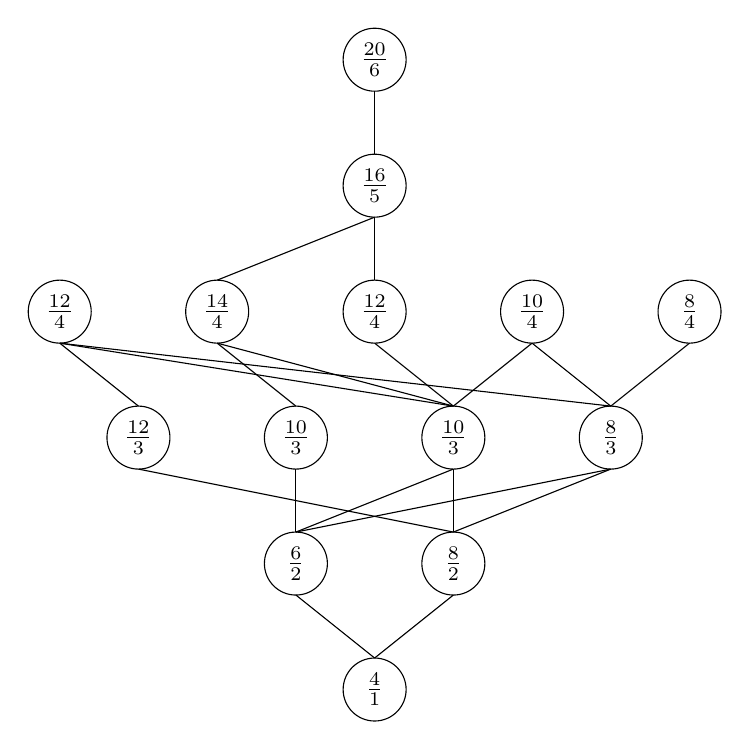
\begin{tikzpicture}
  [scale=.04,auto=left]
  
  \def\X{40}
  \def\Y{0}
  
  \def\x{\X -10}
  \def\y{\Y}
  
  \draw  (\x +10,\y +5) circle [radius=10cm] node {$\frac{4}{1}$};

  \def\x{\X -35}
  \def\y{\Y +40}
    
  \draw  (\x +10,\y +5) circle [radius=10cm] node {$\frac{6}{2}$};
  
  \draw  (\x +10,\y -5) -- (\x +35,\y -25);
  
  \def\x{\X +15}
  \def\y{\Y +40}
    
  \draw  (\x +10,\y +5) circle [radius=10cm] node {$\frac{8}{2}$};
  
  \draw  (\x +10,\y -5) -- (\x -15,\y -25);
  
  \def\x{\X -85}
  \def\y{\Y +80}
    
  \draw  (\x +10,\y +5) circle [radius=10cm] node {$\frac{12}{3}$};
  
  \draw  (\x +10,\y -5) -- (\x +110,\y -25);
  
  \def\x{\X -35}
  \def\y{\Y +80}
    
  \draw  (\x +10,\y +5) circle [radius=10cm] node {$\frac{10}{3}$};
  
  \draw  (\x +10,\y -5) -- (\x +10,\y -25);
  
  \def\x{\X +15}
  \def\y{\Y +80}
    
  \draw  (\x +10,\y +5) circle [radius=10cm] node {$\frac{10}{3}$};
  
  \draw  (\x +10,\y -5) -- (\x +10,\y -25);
  \draw  (\x +10,\y -5) -- (\x -40,\y -25);
  
  \def\x{\X +65}
  \def\y{\Y +80}
    
  \draw  (\x +10,\y +5) circle [radius=10cm] node {$\frac{8}{3}$};
  
  \draw  (\x +10,\y -5) -- (\x -40,\y -25);
  \draw  (\x +10,\y -5) -- (\x -90,\y -25);
  
  \def\x{\X -110}
  \def\y{\Y +120}
    
  \draw  (\x +10,\y +5) circle [radius=10cm] node {$\frac{12}{4}$};
  
  \draw  (\x +10,\y -5) -- (\x +35,\y -25);
  \draw  (\x +10,\y -5) -- (\x +135,\y -25);
  \draw  (\x +10,\y -5) -- (\x +185,\y -25);
  
  \def\x{\X -60}
  \def\y{\Y +120}
    
  \draw  (\x +10,\y +5) circle [radius=10cm] node {$\frac{14}{4}$};
  
  \draw  (\x +10,\y -5) -- (\x +35,\y -25);
  \draw  (\x +10,\y -5) -- (\x +85,\y -25);
  
  \def\x{\X -10}
  \def\y{\Y +120}
    
  \draw  (\x +10,\y +5) circle [radius=10cm] node {$\frac{12}{4}$};
  
  \draw  (\x +10,\y -5) -- (\x +35,\y -25);
  
  \def\x{\X +40}
  \def\y{\Y +120}
    
  \draw  (\x +10,\y +5) circle [radius=10cm] node {$\frac{10}{4}$};
  
  \draw  (\x +10,\y -5) -- (\x +35,\y -25);
  \draw  (\x +10,\y -5) -- (\x -15,\y -25);
  
  \def\x{\X +90}
  \def\y{\Y +120}
    
  \draw  (\x +10,\y +5) circle [radius=10cm] node {$\frac{8}{4}$};
  
  \draw  (\x +10,\y -5) -- (\x -15,\y -25);
  
  \def\x{\X -10}
  \def\y{\Y +160}
    
  \draw  (\x +10,\y +5) circle [radius=10cm] node {$\frac{16}{5}$};
  
  \draw  (\x +10,\y -5) -- (\x +10,\y -25);
  \draw  (\x +10,\y -5) -- (\x -40,\y -25);
  
  \def\x{\X -10}
  \def\y{\Y +200}
    
  \draw  (\x +10,\y +5) circle [radius=10cm] node {$\frac{20}{6}$};
  
  \draw  (\x +10,\y -5) -- (\x +10,\y -25);
\end{tikzpicture}
  \caption{The numbers \(h(G)\) for all cut-minimal graphs on 6 vertices}
  \label{figure2:Figure 2}
\end{figure}


Except for the maximal cut-minimal graphs with maximum number of edges we do not know anything about the remaining classes of cut-minimal graphs until now. The following statements now approach this challenge by providing new classes of cut-minimal graphs in general which do not appear as deletions of those largest maximal cut-minimal graphs.

\begin{lem}\label{lemma8}
Let \(u_1,\ldots,u_t,s_1,\ldots,s_t\in\mathbb{N}\cup\{0\}\), such that for all \(i=1,\ldots,t\) we have
\[
u_i+s_i\leq\sum_{\begin{subarray}{l}j=1\\ j\neq i\end{subarray}}^tu_j+s_j,
\]
then we have:
\[
\sum\limits_{i=1}^ts_i(u_i-\sum_{\begin{subarray}{l}j=1\\ j\neq i\end{subarray}}^tu_j)\leq 0
\]
\begin{proof}
If we have
\[
u_i\leq\sum_{\begin{subarray}{l}j=1\\ j\neq i\end{subarray}}^tu_j
\]
for all \(i=1,\ldots,t\), then we are done, since all \(u_i\)'s and \(s_i\)'s are positive. So, let there exist a \(k\in[t]\), such that
\[
u_k>\sum_{\begin{subarray}{l}j=1\\ j\neq k\end{subarray}}^tu_j
\]
Obviously, there is at most one unique \(u_k\) satisfying this property. Now for all \(i\neq k\) we have
\[
u_i-\sum_{\begin{subarray}{l}j=1\\ j\neq i\end{subarray}}^tu_j\leq -(u_k-\sum_{\begin{subarray}{l}j=1\\ j\neq k\end{subarray}}^tu_j),
\]
and furthermore we have
\[
s_k<\sum_{\begin{subarray}{l}j=1\\ j\neq k\end{subarray}}^ts_j
\]
by assumption and so we get:
\[
\sum_{\begin{subarray}{l}i=1\\ i\neq k\end{subarray}}^ts_i(u_i-\sum_{\begin{subarray}{l}j=1\\ j\neq i\end{subarray}}^tu_j)\leq-s_k(u_k-\sum_{\begin{subarray}{l}j=1\\ j\neq k\end{subarray}}^tu_j)
\]
Hence, we have:
\[
\sum\limits_{i=1}^ts_i(u_i-\sum_{\begin{subarray}{l}j=1\\ j\neq i\end{subarray}}^tu_j)\leq 0
\]
\end{proof}
\end{lem}

\begin{prop}
Let the largest connected component of a graph \(G=([n],E)\) not contain more than \(\frac{n}{2}\) vertices, then \(G\) is cut-minimal.
\begin{proof}
Let \(C_1,\ldots,C_t\subset [n]\) be the connected components of \(G\) and let \(S\subset [n]\), \(S_i\coloneqq S\cap C_i\) and \(U_i\coloneqq C_i\setminus S_i\) for all \(i=1,\ldots,t\). Then we have
\[
|E_G(S,[n]\setminus S)|\leq\sum\limits_{i=1}^t|S_i||U_i|
\] 
and
\[
|NE_G(S,[n]\setminus S)|\geq\sum\limits_{i=1}^t(|S_i|\sum_{\begin{subarray}{l}j=1\\ j\neq i\end{subarray}}^t|U_j|)
\]
So, we have to show that
\[
\sum\limits_{i=1}^t|S_i||U_i|\leq\sum\limits_{i=1}^t(|S_i|\sum_{\begin{subarray}{l}j=1\\ j\neq i\end{subarray}}^t|U_j|),
\]
which is equivalent to
\[
\sum\limits_{i=1}^t|S_i|(|U_i|-\sum_{\begin{subarray}{l}j=1\\ j\neq i\end{subarray}}^t|U_j|)\leq 0,
\]
but this follows directly from Lemma \ref{lemma8}, since by the assumption \(|C_i|\leq\frac{n}{2}\) for all \(i\), we have:
\[
|S_i|+|U_i|=|C_i|\leq\sum_{\begin{subarray}{l}j=1\\ j\neq i\end{subarray}}^t|C_j|=\sum_{\begin{subarray}{l}j=1\\ j\neq i\end{subarray}}^t|S_j|+|U_j|
\]
\end{proof}
\end{prop}

Let us now determine the counterpart of the number \(C_{max}(\Delta^{[n]},1)\), namely the minimal number of edges a non-cut-minimal graph can have, as it was already (more generally) defined in the preceding chapter.

\begin{thm}\label{theorem2}
\(C_{min}(\Delta^{[n]},1)=\left\lceil\frac{n}{2}\right\rceil\)
\begin{proof}
By Proposition \ref{proposition231} we get \(C_{min}(\Delta^{[n]},1)\leq\left\lceil\frac{n}{2}\right\rceil\). On the other hand if we have a graph \(G=([n],E)\) with \(|E|=\left\lceil\frac{n}{2}\right\rceil-1\), then it must be cut-minimal, since for any set of vertices \(S\subset[n]\), such that \(|S|<\frac{n}{2}\) we have \(\frac{|S|(n-|S|)}{2}\leq\frac{(|S|+1)(n-(|S|+1))}{2}\) and we have \(|E|=\left\lceil\frac{n}{2}\right\rceil-1=\left\lfloor\frac{n-1}{2}\right\rfloor\), so inductively \(|E(S,[n]\setminus S)|\leq\frac{|S|(n-|S|)}{2}\) holds for every \(S\subset [n]\) such that \(|S|\leq\frac{n}{2}\). Hence, we get \(C_{min}(\Delta^{[n]},1)\geq\left\lceil\frac{n}{2}\right\rceil\) and we are done.
\end{proof}
\end{thm}

Obviously, \(\mathcal{C}_1(\Delta^{[n]})\) contains all simplices of dimension strictly lower than\\
\(C_{min}(\Delta^{[n]},1)-1\), which leads to the following observation.

\begin{cor}
\(H_k(\mathcal{C}_1(\Delta^{[n]}))\cong 0\) for all \(1\leq k\leq\left\lceil\frac{n}{2}\right\rceil-3\)
\begin{proof}
By Theorem \ref{theorem2} \(\mathcal{C}_1(\Delta^{[n]})\) has a full \(k\)-skeleton for all \(k\leq\left\lceil\frac{n}{2}\right\rceil-2\) and we are done. 
\end{proof}
\end{cor}

Since adding a vertex to a cut-minimal graph will always preserve its property to be cut-minimal (see Lemma \ref{lemma132}), we can define the following natural embedding:

\begin{align}
i_n:CMG(n)&\longrightarrow CMG(n+1)\notag \\
([n],E)&\longmapsto ([n+1],E)\notag
\end{align}

Note, that the embedding \(i_n\) is just the graphic version of the more general embedding \(i_n^k\) for cochains from the preceding chapter, restricted to cut-minimal graphs.\\
Now, the first thing we see is that maximality of cut-minimal graphs always becomes destroyed by embedding them.

\begin{prop}
Let \(G\in MAX(n)\), then we have \(i_n(G)\notin MAX(n+1)\).
\begin{proof}
Let \(G=([n],E)\in MAX(n)\). If \(n\) is odd, Theorem \ref{theorem1} gives
\[
|E|\leq\frac{n^2-2n+1}{4}<\frac{n^2-n}{4}=\frac{n\frac{n-1}{2}}{2},
\]
so there exists a \(v\in [n]\), such that \(\deg_G(v)<\frac{n-1}{2}\). Now define\\
\(G'\coloneqq ([n+1],E\cup\{(v,n+1)\})\) and let \(S\subset [n+1]\), such that \(1\leq |S|\leq\frac{n+1}{2}\), then we have
\begin{align}
|E_{G'}(S,[n+1]\setminus S)|&\leq |E_G(S\setminus\{n+1\},[n]\setminus S)|+1\notag\\
&\leq\frac{|S|(n-|S|)}{2}+1\notag\\
&=\frac{|S|(n+\frac{2}{|S|}-|S|)}{2}\notag\\
&\leq\frac{|S|(n+1-|S|)}{2},\notag
\end{align}
for all \(S\subset [n+1]\), such that \(|S|\geq 2\). For \(|S|=1\), the upper condition is also satisfied, since we have \(\deg_G(v)<\frac{n-1}{2}\).\\
Hence, \(G'\) is cut-minimal and so we have \(i_n(G)=([n+1],E)\notin MAX(n+1)\).\\
If \(n\) is even, define \(G'\coloneqq ([n+1],E\cup (v,n+1))\) for an arbitrary \(v\in [n]\). Then by the same calculations as in the first part we have
\[
|E_{G'}(S,[n+1]\setminus S)|\leq\frac{|S|(n+1-|S|)}{2},
\]
for all \(S\subset [n+1]\) such that \(|S|\geq 2\), and for \(|S|=1\) we have:
\begin{align}
|E_{G'}(S,[n+1]\setminus S)|&\leq\text{max}\{\deg_{G'}(w):w\in[n+1]\}\notag\\
&\leq\left\lfloor\frac{n-1}{2}\right\rfloor +1\notag\\
&=\frac{n-2}{2}+1=\frac{n}{2}=\frac{(n+1)-1}{2}\notag
\end{align}
Hence, \(G'\) is cut-minimal and \(i_n(G)\notin MAX(n+1)\).
\end{proof}
\end{prop}

\section{Basic definitions and properties of Cheeger graphs}

The following definition is completely adopted from \cite{1} (Definition 2.6).
\begin{defi}\label{definition1}
Consider a graph \(G=([n],E)\), then we set:
\begin{small}
\[
T(G)\coloneqq \{(v,e)\: :\: v\in [n]\text{, }e=(w,u)\in E\text{, }v\notin e\text{, }|\{(v,w),(v,u),(w,u)\}\cap E\}|\text{ is odd}\}
\]
\end{small}
We have
\[
|T(G)|=\sum\limits_{e\in E}t(e),
\]
where for an edge \(e=(v,w)\in E\), we set
\[
t(e)\coloneqq \sum\limits_{\begin{subarray}{l}u\in[n]\\ u\neq v,w\end{subarray}}\tau_e(u),
\]
with
\begin{equation}
\tau_e(u)\coloneqq 
\begin{cases}
1,&\text{ if }(v,u),(w,u)\notin E\notag\\
\frac{1}{3},&\text{ if }(v,u),(w,u)\in E\notag\\
0,&\text{ otherwise}\notag
\end{cases}
\end{equation}
Furthermore, we define
\[
h(G)\coloneqq \frac{|T(G)|}{|E|},
\]
and call a cut-minimal graph \(G=([n],E)\) a \textbf{Cheeger graph}\index{Cheeger graph}, if
\[
h(G)=\min\limits_{G'\in CMG(n)}h(G')
\]
The \textbf{first Cheeger constant of a simplex}\index{Cheeger constant} is defined by
\[
h_1(\Delta^{[n]})\coloneqq h(G),
\]
where \(G\) is some Cheeger graph on \(n\) vertices.
\end{defi}
We already know by \cite{1} (Theorem 4.1 and Corollary 4.3) that we have \(\frac{n}{3}\leq h_1(\Delta{[n]})\leq\left\lceil\frac{n}{3}\right\rceil\) and the lower bound is archieved if \(n\) is not a power of \(2\). If two graphs \(G\) and \(G'\) belong to the same isomorphism class, we obviously have \(|T(G)|=|T(G')|\) and \(h(G)=h(G')\), so taking up the example from the preceding section, Figure \ref{figure3:Figure 3} shows the numbers \(h(G)\) for all cut-minimal graphs on \(6\) vertices with the same partially ordering as in Figure \ref{figure2:Figure 2} and we can see that there is one isomorphism class of Cheeger graphs attaining the Cheeger constant \(\frac{8}{4}\).

\begin{figure}[ht]
\centering
\begin{tikzpicture}
  \matrix (m) [matrix of math nodes, row sep=5em, column sep=1.5em]
    { \cdots & C^{k-1}(\Delta^{[n]},\mathbb{Z}_2) & C^{k}(\Delta^{[n]},\mathbb{Z}_2) & C^{k+1}(\Delta^{[n]},\mathbb{Z}_2) & \cdots \\
      \cdots & C^{k-1}(\Delta^{[n+1]},\mathbb{Z}_2) & C^{k}(\Delta^{[n+1]},\mathbb{Z}_2) & C^{k+1}(\Delta^{[n+1]},\mathbb{Z}_2) & \cdots \\ };
  { [start chain] \chainin (m-1-1);
    \chainin (m-1-2);
    { [start branch=A] \chainin (m-2-2)
        [join={node[right,labeled] {i}}];}
    \chainin (m-1-3) [join={node[above,labeled] {\delta}}];
    { [start branch=B] \chainin (m-2-3)
        [join={node[right,labeled] {i}}];}
    \chainin (m-1-4) [join={node[above,labeled] {\delta}}];
    { [start branch=C] \chainin (m-2-4)
        [join={node[right,labeled] {i}}];}
    \chainin (m-1-5); }
  { [start chain] \chainin (m-2-1);
    \chainin (m-2-2);
    \chainin (m-2-3) [join={node[above,labeled] {\delta}}];
    \chainin (m-2-4) [join={node[above,labeled] {\delta}}];
    \chainin (m-2-5); }
  { [start chain] \chainin (m-1-2);
  	\chainin (m-2-3) [join={node[above,labeled] {\varepsilon}}]; }
  { [start chain] \chainin (m-1-3);
  	\chainin (m-2-4) [join={node[above,labeled] {\varepsilon}}]; }
\end{tikzpicture}
 \caption{Cochain complexes with coning maps}
 \label{figure3:Figure 3}
\end{figure}


\section{A restriction on the size of connected components in\\ Cheeger graphs}
The following statement restricts the shape of Cheeger graphs in terms of the sizes of their connected components.

\begin{prop}
Let \(G=([n],E)\) be a Cheeger graph, then \(G\) must have a connected component of size at least \(n-\left\lceil\frac{n}{3}\right\rceil\).
\begin{proof}
Let \(C\subseteq [n]\) be the largest connected component of \(G\), then we obviously have
\[
\left\lceil\frac{n}{3}\right\rceil\geq h(G)\geq \frac{|E|(n-|C|)}{|E|}=n-|C|,
\]
which is equivalent to
\[
|C|\geq n-\left\lceil\frac{n}{3}\right\rceil
\]
\end{proof}
\end{prop}

A direct consequence of the preceding statement is, that for \(n\geq 6\) a Cheeger graph can never appear as a subgraph of a largest cut-minimal graph such as constructed in the proof of Proposition \ref{proposition3}.



\section{Embeddings of Cheeger graphs}

Based on the fact from the preceding chapter (see Lemma \ref{lemma132}) that adding a vertex to a cut-minimal graph will always result in a cut-minimal graph again, we will now study the consequences of adding a vertex to a Cheeger graph. It will turn out that the resulting graph will not be a Cheeger graph anymore. Using this fact we will be able to find a lower bound on the number of edges in Cheeger graphs. The following statement is just the graphic version of Proposition \ref{proposition113}.

\begin{prop}\label{proposition351}
Let \(G=([n],E)\) be a cut-minimal graph, then we have:
\[
h(i_n(G))=h(G)+1
\]
\end{prop}

\begin{prop}\label{proposition352}
Let \(G\in CMG(n)\), then \(i_n(G)\in CMG(n+1)\) is not a Cheeger graph.
\begin{proof}
Without loss of generality let \(G\) be a Cheeger graph. Otherwise, there exists a graph \(G'\in CMG(n)\), such that \(h(G')<h(G)\), so by Proposition \ref{proposition351} we get:
\[
h(i_n(G'))=h(G')+1<h(G)+1=h(i_n(G))
\]
Let now \(n+1\) not be a power of \(2\). Since we have \(h(G)\geq\frac{n}{3}\), by Proposition \ref{proposition351} we get
\[
h(i_n(G))\geq\frac{n}{3}+1=\frac{n+3}{3}>\frac{n+1}{3},
\]
so \(i_n(G)\) can not be a Cheeger graph. On the other hand if \(n+1\) is a power of \(2\), then \(n\) can not be a power of \(2\) and we have:
\[
h(i_n(G))=h(G)+1=\frac{n}{3}+1\geq\left\lceil\frac{n+1}{3}\right\rceil
\]
But by \cite{1} (Theorem 4.6) we have that \(h_1(\Delta^{[n+1]})<\left\lceil\frac{n+1}{3}\right\rceil\) holds if \(n+1\) is a power of \(2\), so \(i_n(G)\) can not be a Cheeger graph.
\end{proof}
\end{prop}

We can now calculate a lower bound for the number of edges in Cheeger graphs.

\begin{prop}
Let \(G=([n],E)\) be a Cheeger graph, then we have \(|E|\geq\left\lceil\frac{n-1}{2}\right\rceil\).
\begin{proof}
Assume we have \(|E|<\left\lceil\frac{n-1}{2}\right\rceil\). Then by Theorem \ref{theorem2} and since \(G\) must contain an isolated vertex, there exists a graph \(G'\in CMG(n-1)\) such that \(i_{n-1}(G')=G\), so by Proposition \ref{proposition352} \(G\) can not be a Cheeger graph and we are done.
\end{proof}
\end{prop}

\section{The case when n is a power of 2}

From \cite{1} (Corollary 4.3) we know that \(h(\Delta^{[n]})>\frac{n}{3}\) can only be valid, if \(n\) is a power of \(2\). An interesting question is, if this inequality is always strict for such \(n\). For a graph \(G=([n],E)\) and a vertex \(v\in [n]\) let us introduce the notation\\
\(A_v\coloneqq \{w\in [n]:(v,w)\in E\}\), so we have \(|A_v|=\deg_G(v)\). The following useful fact was given by Kozlov (see \cite{1}, Section 6.3).

\begin{lem}\label{lemma11:2}
Let \(G=([n],E)\) be a cut-minimal graph, then we have \(h(G)=\frac{n}{3}\) if and only if for each vertex \(v\in [n]\) we have \(|E(A_v\text{, }[n]\setminus A_v)|=|NE(A_v\text{, }[n]\setminus A_v)|\).
\end{lem}

We can now make a statement about the possible degrees a vertex in a Cheeger graph on \(n=2^t\) vertices can attain, assuming the first Cheeger constant exactly equals \(\frac{n}{3}\).

\begin{prop}\label{proposition321}
Let \(n=2^t\) and \(G=([n],E)\) be a cut-minimal graph, such that \(h(G)=\frac{n}{3}\). Then for each vertex \(v\in [n]\) we have \(|A_v|\in\left\{0\leq i\leq\frac{n-4}{2}:i\text{ is even }\right\}\setminus\{2\}\).
\begin{proof}
The proof of the fact, that \(|A_v|\) is even can be found in \cite{1} (Section 6.3). Since \(G\) is cut-minimal and \(n=2^t\), we have:
\[
|A_v|=|E(\{v\}\text{, }[n]\setminus\{v\})|\leq\left\lfloor\frac{n-1}{2}\right\rfloor=2^{t-1}-1
\]
But \(2^{t-1}-1\) is always odd, so we get:
\begin{equation}\label{equation2}
|A_v|\leq 2^{t-1}-2=\frac{n-4}{2}
\end{equation}
Now, assume there exists a \(v\in [n]\), such that \(|A_v|=2\), then by Lemma \ref{lemma11:2} we have
\[
|E(A_v\text{, }[n]\setminus A_v)|=\frac{2(n-2)}{2}=n-2,
\]
so there must exist a \(w\in A_v\), such that \(|A_w|\geq\frac{n-2}{2}=\frac{2^t-2}{2}=2^{t-1}-1\), but this is a contradiction to \ref{equation2}.
\end{proof}
\end{prop}

\begin{expl}
In \cite{1} (Section 6.3) Kozlov already used the fact, that a vertex in a graph satisfying the conditions of the preceding proposition can not attain an odd degree to prove the strict bound \(h(\Delta^{[8]})>\frac{8}{3}\). Applying the preceding slightly stronger proposition we get this result immediately, since then every vertex in a Cheeger graph \(G=([8],E)\), satisfying \(h(G)=\frac{8}{3}\) must attain degree \(0\), which obviously leads to a contradiction.
\end{expl}

Furthermore, we can make some statements about the graph structure of \(G=([n],E)\) according to the degrees of its vertices if \(n\) is a power of \(2\) and \(h(G)=\frac{n}{3}\).

\begin{lem}\label{lemma362}
Let \(n=2^t\) and \(G=([n],E)\) be a cut-minimal graph, such that \(h(G)=\frac{n}{3}\). Then for each vertex \(v\in [n]\), such that \(\deg_G(v)=4\) we have \(\deg_G(w)=\frac{n-4}{2}\) for all \(w\in A_v\) and \(|E(A_v,A_v)|=0\).
\begin{proof}
Let \(v\in [n]\) such that \(\deg_G(v)=4\), then by Lemma \ref{lemma11:2} we have
\[
|E(A_v,[n]\setminus A_v)|=\frac{|A_v|(n-|A_v|)}{2}=\frac{4(n-4)}{2},
\]
so since \(\frac{n-4}{2}\) is the maximum possible degree of a vertex in \(G\) by Proposition \ref{proposition321} we have \(\deg_G(w)=\frac{n-4}{2}\) for all \(w\in A_v\) and \(|E(A_v,A_v)|=0\).
\end{proof}
\end{lem}

\begin{defi}
Let \(G=([n],E)\) be a graph, then a subset \(T=\{v,w,u\}\subseteq [n]\) is called a \textbf{triangle} if \((v,w),(v,u),(w,u)\in E\). The number of triangles in \(G\) is denoted by \(t(G)\).
\end{defi}

The following statement describes the relation among the degrees of the vertices and the number of triangles in a cut-minimal graph \(G\) attaining \(h(G)=\frac{n}{3}\).

\begin{lem}\label{lemma363}
Let \(G=([n],E)\) be a cut-minimal graph, such that \(h(G)=\frac{n}{3}\), then we have:
\[
t(G)=\frac{1}{4}\sum\limits_{v\in [n]}\deg_G(v)^2-\frac{n}{12}\sum\limits_{v\in [n]}\deg_G(v)
\]
\begin{proof}
Rearranging the formula from Definition \ref{definition1} gives
\[
|T(G)|=\sum\limits_{v\in [n]}t(v),
\]
where for a vertex \(v\in [n]\) we set
\[
t(v)\coloneqq\sum\limits_{\begin{subarray}{l}e\in E \\ v\notin e\end{subarray}}\tau_e(v),
\]
with \(\tau_e(v)\) defined exactly as in Definition \ref{definition1}.\\
So, applying Lemma \ref{lemma11:2} we get
\[
t(v)=|E|-\frac{\deg_G(v)(n-\deg_G(v))}{2}-\frac{2}{3}t_v,
\]
where \(t_v\) denotes the number of triangles which contain \(v\).\\
Since every triangle contains exactly \(3\) vertices, overall we get:
\[
|T(G)|=\sum\limits_{v\in [n]}|E|-\frac{\deg_G(v)(n-\deg_G(v))}{2}-2t(G)
\]
Furthermore, we know that \(|E|=\frac{1}{2}\sum\limits_{v\in [n]}\deg_G(v)\) and by assumption we have \(h(G)=\frac{|T(G)|}{|E|}=\frac{n}{3}\), so rearranging the preceding formula gives:
\[
t(G)=\frac{1}{4}\sum\limits_{v\in [n]}\deg_G(v)^2-\frac{n}{12}\sum\limits_{v\in [n]}\deg_G(v)
\]
\end{proof}
\end{lem}

Let us now consider the case \(n=16\). This case seems to be much more complicated than the case \(n=8\), but nevertheless we can prove the strict inequality \(h(\Delta^{[16]})>\frac{16}{3}\) and hopefully use some ideas from the proof to get hands on the general conjecture that \(h(\Delta^{[n]})>\frac{n}{3}\) holds if and only if \(n\) is a power of \(2\).

\begin{lem}\label{lemma364}
Let \(G=([16],E)\) be cut-minimal, such that \(h(G)=\frac{16}{3}\) and \(v\in [16]\), such that \(\deg_G(v)=6\), then we have \(|E(A_v,A_v)|\in\{0,1,2,3\}\), for every \(e=(w,u)\in E(A_v,A_v)\) we have \(\deg_G(w)=6\) and \(\deg_G(u)=6\) and for \(e_1,e_2\in E(A_v,A_v)\) (\(e_1\neq e_2\)) we have \(e_1\cap e_2=\emptyset\).
\begin{proof}
By Lemma \ref{lemma11:2} we have \(|E(A_v,[16]\setminus A_v)|=30\) and by Proposition \ref{proposition321} we have \(\deg_G(w)\in\{4,6\}\) for every \(w\in A_v\), so if we have \(\deg_G(w)=6\) for all \(w\in A_v\) we get \(\sum\limits_{w\in A_v}\deg_G(w)=36\) which implies that \(|E(A_v,A_v)|=3\). By the same argument for each vertex \(w\in A_v\) such that \(\deg_G(w)=4\) there is one edge less in \(E(A_v,A_v)\) such that \(|E(A_v,A_v)|=0\) if and only if \(3\) vertices in \(A_v\) attain degree \(4\) and \(3\) vertices in \(A_v\) attaing degree \(6\), since then we have \(\sum\limits_{w\in A_v}\deg_G(w)=30\). Now assume there exists an edge \(e=(w,u)\in E(A_v,A_v)\) such that \(\deg_G(w)=4\), then \((u,v)\in E(A_w,A_w)\) which is a contradiction to Lemma \ref{lemma362}. The proof for \(\deg_G(u)=6\) is analogous. Finally denote \(A_v=\{w_1,w_2,w_3,w_4,w_5,w_6\}\) and assume \((w_1,w_2),(w_2,w_3)\in E(A_v,A_v)\). Then there exists at most one more edge in \(E(A_v,A_v)\) and by the preceding result we have \(\deg_G(w_2)=6\), so setting \(S\coloneqq\{w_1,w_3,w_4,w_5,w_6\}\) gives \(|E(S,[16]\setminus S)|\geq 28>\frac{5(16-5)}{2}\) and \(G\) is not cut-minimal anymore.
\end{proof}
\end{lem}

Summarizing the statements of the preceding lemma just means that for a cut-minimal graph \(G=([16],E)\), such that \(h(G)=\frac{16}{3}\), for every \(v\in [16]\) with \(\deg_G(v)=6\) we have one of the following shapes (up to isomorphy) for \(A_v\), where the numbers at the vertices denote their degrees (see Figure \ref{figure8:Figure 8}).

\newpage

\begin{figure}[ht]
\centering
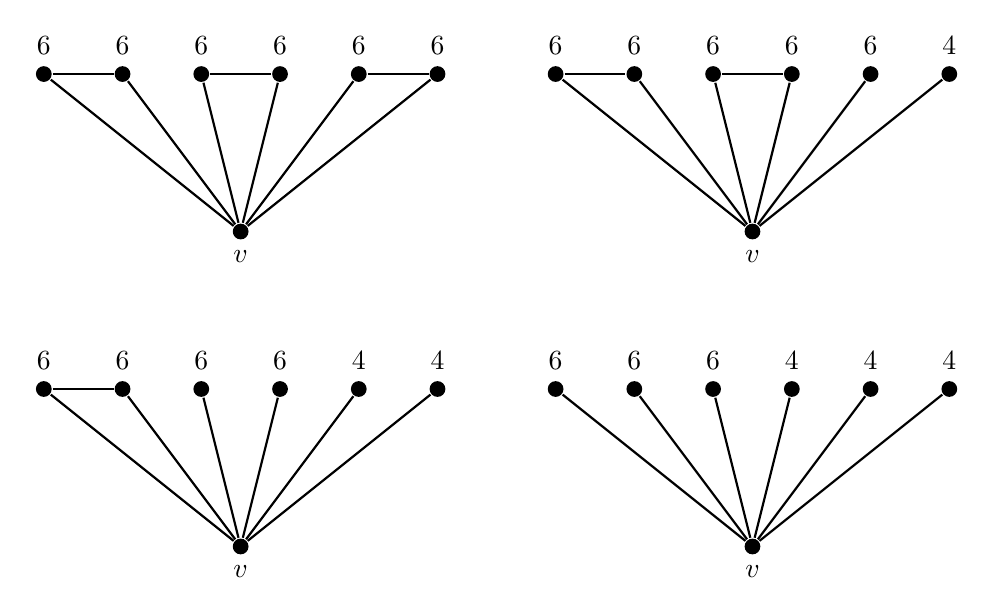
\begin{tikzpicture}[
       thick,
       acteur/.style={
         circle,
         fill=black,
         thick,
         inner sep=2pt,
         minimum size=0.2cm
       }
     ]

       \node (v) at (-3.5,0) [acteur,label=below:$v$]{};
       \node (w1) at (-6,2)[acteur,label=above:$6$]{}; 
       \node (w2) at (-5,2) [acteur,label=above:$6$]{}; 
       \node (w3) at (-4,2) [acteur,label=above:$6$]{};
       \node (w4) at (-3,2) [acteur,label=above:$6$]{};
       \node (w5) at (-2,2) [acteur,label=above:$6$]{};
       \node (w6) at (-1,2) [acteur,label=above:$6$]{};
  
       \draw (v) -- (w1);
       \draw (v) -- (w2);
       \draw (v) -- (w3);
       \draw (v) -- (w4);
       \draw (v) -- (w5);
       \draw (v) -- (w6);
       
       \draw (w1) -- (w2);
       \draw (w3) -- (w4);
       \draw (w5) -- (w6);
       
       
       \node (v) at (3,0) [acteur,label=below:$v$]{};
       \node (w1) at (0.5,2)[acteur,label=above:$6$]{}; 
       \node (w2) at (1.5,2) [acteur,label=above:$6$]{}; 
       \node (w3) at (2.5,2) [acteur,label=above:$6$]{};
       \node (w4) at (3.5,2) [acteur,label=above:$6$]{};
       \node (w5) at (4.5,2) [acteur,label=above:$6$]{};
       \node (w6) at (5.5,2) [acteur,label=above:$4$]{};
  
       \draw (v) -- (w1);
       \draw (v) -- (w2);
       \draw (v) -- (w3);
       \draw (v) -- (w4);
       \draw (v) -- (w5);
       \draw (v) -- (w6);
       
       \draw (w1) -- (w2);
       \draw (w3) -- (w4);
       
       
       \node (v) at (-3.5,-4) [acteur,label=below:$v$]{};
       \node (w1) at (-6,-2)[acteur,label=above:$6$]{}; 
       \node (w2) at (-5,-2) [acteur,label=above:$6$]{}; 
       \node (w3) at (-4,-2) [acteur,label=above:$6$]{};
       \node (w4) at (-3,-2) [acteur,label=above:$6$]{};
       \node (w5) at (-2,-2) [acteur,label=above:$4$]{};
       \node (w6) at (-1,-2) [acteur,label=above:$4$]{};
  
       \draw (v) -- (w1);
       \draw (v) -- (w2);
       \draw (v) -- (w3);
       \draw (v) -- (w4);
       \draw (v) -- (w5);
       \draw (v) -- (w6);
       
       \draw (w1) -- (w2);
    
       
       \node (v) at (3,-4) [acteur,label=below:$v$]{};
       \node (w1) at (0.5,-2)[acteur,label=above:$6$]{}; 
       \node (w2) at (1.5,-2) [acteur,label=above:$6$]{}; 
       \node (w3) at (2.5,-2) [acteur,label=above:$6$]{};
       \node (w4) at (3.5,-2) [acteur,label=above:$4$]{};
       \node (w5) at (4.5,-2) [acteur,label=above:$4$]{};
       \node (w6) at (5.5,-2) [acteur,label=above:$4$]{};
  
       \draw (v) -- (w1);
       \draw (v) -- (w2);
       \draw (v) -- (w3);
       \draw (v) -- (w4);
       \draw (v) -- (w5);
       \draw (v) -- (w6);
       

\end{tikzpicture}
  \caption{Possible shapes of $A_v$ if $\deg_G(v)=6$}
  \label{figure8:Figure 8}
\end{figure}


\begin{lem}\label{lemma365}
Let \(G=([16],E)\) be a cut-minimal graph, such that \(h(G)=\frac{16}{3}\) and \(T=\{v_1,v_2,v_3\}\subset [16]\) be a triangle, then for every \(w\in [16]\setminus T\) satisfying \(\deg_G(w)\neq 0\) there exists an \(i\in\{1,2,3\}\), such that \((v_i,w)\in E\).
\begin{proof}
Assume there exists a \(w\in [16]\setminus T\), such that \((v_i,w)\notin E\) for all \(i=1,2,3\). First consider the case \(\deg_G(w)=6\). There must exist a \(v_i\in T\) such that \(|E(\{v_i\},A_w)|\leq 2\), since otherwise we had a second triangle sharing an edge with \(T\) which is a contradiction to Lemma \ref{lemma364}. Now, set \(S\coloneqq A_w\cup\{v_i\}\), then we have \(|E(S,[16]\setminus S)|\geq 32>\frac{7(16-7)}{2}\), since we have \(|E(A_w,A_w)|=30\) by Lemma \ref{lemma11:2} and \(\deg_G(v_i)=6\) by Lemma \ref{lemma362}. Thus, \(G\) would not be cut-minimal anymore. Now, consider the case \(\deg_G(w)=4\), then by the same argument there must exist a \(v_i\in T\) such that \(|E(\{v_i\},A_w)|\leq 1\) and setting \(S\coloneqq A_w\cup\{v_i\}\) we get \(|E(S,[16]\setminus S)|\geq 28>\frac{5(16-5)}{2}\), since \(|E(A_w,A_w)|=24\) by Lemma \ref{lemma11:2} and \(\deg_G(v_i)=6\) by Lemma \ref{lemma362}. Hence, \(G\) would not be cut-minimal anymore again.
\end{proof}
\end{lem}

\begin{lem}\label{lemma366}
Let \(G=([16],E)\) be a cut-minimal graph, such that \(h(G)=\frac{16}{3}\) and \(T=\{v_1,v_2,v_3\}\subset [16]\) be a triangle, then we have
\[
|\{v\in [16]:\deg_G(v)\neq 0\}|=15
\]
\begin{proof}
By Lemma \ref{lemma362} we have \(\deg_G(v_i)=6\) for all \(i=1,2,3\) and by Lemma \ref{lemma364} the sets \(A_{v_i}\setminus T\) are pairwise disjoint, since otherwise we had a second triangle sharing an edge with \(T\), so we have \(|\{v\in [16]:\deg_G(v)\neq 0\}|\geq 15\). But since for every \(w\in [16]\setminus T\), satisfying \(\deg_G(w)\neq 0\) there exists an \(i\in\{1,2,3\}\), such that \((v_i,w)\in E\) by Lemma \ref{lemma365}, we have \(|\{v\in [16]:\deg_G(v)\neq 0\}|=15\).
\end{proof}
\end{lem}

\begin{lem}\label{lemma367}
Let \(G=([16],E)\) be a cut-minimal graph, such that \(h(G)=\frac{16}{3}\) and \(v,w\in [16]\), such that \(\deg_G(v)=\deg_G(w)=4\), then we have \(A_v\cap A_w\neq\emptyset\).
\begin{proof}
Assume we have \(A_v\cap A_w=\emptyset\) and set \(S:=A_v\cup\{w\}\). By Lemma \ref{lemma11:2} we get \(|E(S,[16]\setminus S)|=28\), but this is a contradiction to the cut-minimality of \(G\) since we have \(\left\lfloor\frac{5(16-5)}{2}\right\rfloor=27\).
\end{proof}
\end{lem}

\begin{lem}\label{lemma368}
Let \(G=([16],E)\) be a cut-minimal graph, such that \(h(G)=\frac{16}{3}\), \(v\in [16]\) such that \(\deg_G(v)=6\) and \(u\in [16]\setminus (\{v\}\cup A_v)\), such that \(\deg_G(u)=6\), then we have \(|E(\{u\},A_v)|\geq 3\).
\begin{proof}
Assume \(|E(\{u\},A_v)|\leq 2\) and set \(S\coloneqq A_v\cup\{u\}\), then by Lemma \ref{lemma11:2} we have \(|E(S,[16]\setminus S)|\geq 32\), but this is a contradiction to the cut-minimality of \(G\) since we have \(\left\lfloor\frac{7(16-7)}{2}\right\rfloor=31\).
\end{proof}
\end{lem}

\begin{thm}\label{theoremn=16}
\(h(\Delta^{[16]})>\frac{16}{3}\)
\begin{proof}
Assume \(G=([16],E)\) is a cut-minimal graph, such that \(h(G)=\frac{16}{3}\). By Proposition \ref{proposition321} we have \(\deg_G(v)\in\{0,4,6\}\) for every vertex \(v\in [16]\). Then Lemma \ref{lemma363} gives the relation

\begin{equation}\label{equation361}
t(G)=s-\frac{4}{3}f,
\end{equation}

where \(s\) denotes the number of vertices attaining degree \(6\) and \(f\) denotes the number of vertices attaining degree \(4\) in \(G\). It follows that \(f\) has to be a multiple of \(3\) and \(s\geq\frac{4}{3}f\), since \(t(G)\) is a positive integer. Since the sum of \(s\) and \(f\) can not exceed \(16\) we will depart the proof into the possible cases \(f=0\), \(f=3\) and \(f=6\).\\
Let us begin with the case \(f=0\). Let \(v\in [16]\), such that \(\deg_G(v)=6\) and denote \(A_v=\{w_1,w_2,w_3,w_4,w_5,w_6\}\) such that \((w_1,w_2),(w_3,w_4),(w_5,w_6)\in E(A_v,A_v)\) according to Lemma \ref{lemma364}. Now, by Lemma \ref{lemma364} we have \(A_{w_1}=\{v,w_2,u_1,u_2,u_3,u_4\}\) such that \(u_1,u_2,u_3,u_4\notin A_v\cup \{v\}\) and \((v,w_2),(u_1,u_2),(u_3,u_4)\in E(A_{w_1},A_{w_1})\). Setting \(W_1\coloneqq\{w_3,w_4\}\) and \(W_2\coloneqq\{w_5,w_6\}\) we have \(|E(\{u_i\},W_1)|=1\) and\\
\(|E(\{u_i\},W_2)|=1\) for all \(i=1,2,3,4\) by Lemma \ref{lemma365} and \ref{lemma364}. Analogously, setting \(U_1\coloneqq\{u_1,u_2\}\) and \(U_2\coloneqq\{u_3,u_4\}\) we have \(|E(\{w_i\},U_1)|=1\) and \(|E(\{w_i\},U_2)|=1\) for all \(i=3,4,5,6\) by Lemma \ref{lemma365} and \ref{lemma364}. Thus, there must exist a set \(S=\{w_2,w_i,w_j,u_k,u_l\}\) with \(w_i\in W_1\), \(w_j\in W_2\), \(u_k\in U_1\) and \(u_l\in U_2\), such that \(|E(S,S)|\leq 1\) which implies that \(|E(S,[16]\setminus S)|\geq 28\), so \(G\) is not cut-minimal anymore, since we have \(\left\lfloor\frac{5(16-5)}{2}\right\rfloor=27\). For more clarity Figure \ref{figure9:Figure 9} gives a sketch about the relevant parts of the graph we constructed within the proof.\\

\begin{figure}[H]
\centering
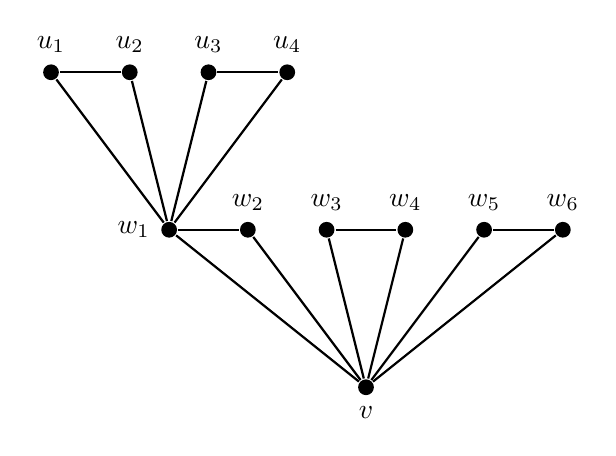
\begin{tikzpicture}[
       thick,
       acteur/.style={
         circle,
         fill=black,
         thick,
         inner sep=2pt,
         minimum size=0.2cm
       }
     ]

       \node (v) at (-3.5,0) [acteur,label=below:$v$]{};
       \node (w1) at (-6,2) [acteur,label=left:$w_1$]{}; 
       \node (w2) at (-5,2) [acteur,label=above:$w_2$]{}; 
       \node (w3) at (-4,2) [acteur,label=above:$w_3$]{};
       \node (w4) at (-3,2) [acteur,label=above:$w_4$]{};
       \node (w5) at (-2,2) [acteur,label=above:$w_5$]{};
       \node (w6) at (-1,2) [acteur,label=above:$w_6$]{};
       \node (u1) at (-7.5,4) [acteur,label=above:$u_1$]{};
  	   \node (u2) at (-6.5,4) [acteur,label=above:$u_2$]{};
  	   \node (u3) at (-5.5,4) [acteur,label=above:$u_3$]{};
  	   \node (u4) at (-4.5,4) [acteur,label=above:$u_4$]{};
  	   
       \draw (v) -- (w1);
       \draw (v) -- (w2);
       \draw (v) -- (w3);
       \draw (v) -- (w4);
       \draw (v) -- (w5);
       \draw (v) -- (w6);
       
       \draw (w1) -- (w2);
       \draw (w3) -- (w4);
       \draw (w5) -- (w6);
       
       \draw (w1) -- (u1);
       \draw (w1) -- (u2);
       \draw (w1) -- (u3);
       \draw (w1) -- (u4);
       
       \draw (u1) -- (u2);
       \draw (u3) -- (u4);
       

\end{tikzpicture}
  \caption{The case $f=0$}
  \label{figure9:Figure 9}
\end{figure}


Now, consider the case \(f=3\). Let \(v\in [16]\), such that \(\deg_G(v)=4\) and denote \(A_v=\{w_1,w_2,w_3,w_4\}\). By Lemma \ref{lemma362} we have \(\deg_G(w_i)=6\) for all \(i=1,2,3,4\), so by Lemma \ref{lemma362} and \ref{lemma364} we get \(|\{w\in [16]:\deg_G(w)=6\}|>4\). Applying Equation \ref{equation361} there exists a triangle in \(G\), so by Lemma \ref{lemma366} we have\\
\(|\{v\in [16]:\deg_G(v)\neq 0\}|=15\) and we can apply Equation \ref{equation361} again. Thus, we get \(t(G)=8\). By Lemma \ref{lemma365} and \ref{lemma362} for every triangle \(T\subset [16]\) we have \(|T\cap A_v|=1\), but by Lemma \ref{lemma364} every vertex in \(A_v\) can be contained in at most two triangles, so by \(t(G)=8\) every vertex in \(A_v\) is contained in exactly two triangles, which implies that \(\deg_G(u)=6\) for all \(u\in A_{w_i}\setminus\{v\}\) and all \(i=1,2,3,4\) by Lemma \ref{lemma364}. Now, let \(v'\in [16]\) be another vertex satisfying \(\deg_G(v')=4\), which exists by the assumption \(f=3\). By the preceding result, we have \(A_v\cap A_{v'}=\emptyset\), which is a contradiction to Lemma \ref{lemma367}. Figure \ref{figure10:Figure 10} gives a sketch about the relevant parts of the graph we constructed within the proof again, where the numbers at the vertices denote their degrees.\\

\begin{figure}[H]
\centering
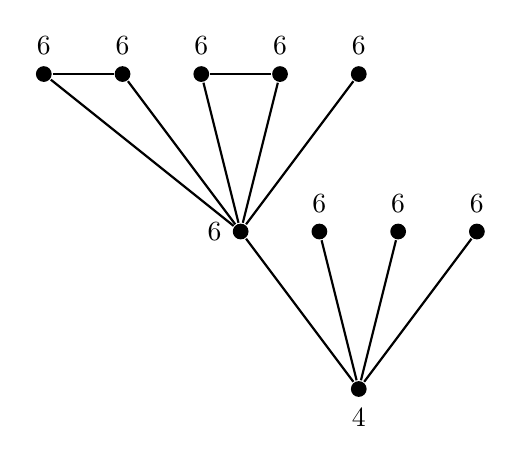
\begin{tikzpicture}[
       thick,
       acteur/.style={
         circle,
         fill=black,
         thick,
         inner sep=2pt,
         minimum size=0.2cm
       }
     ]

       \node (v) at (-3.5,0) [acteur,label=below:$4$]{};
       \node (w1) at (-5,2) [acteur,label=left:$6$]{}; 
       \node (w2) at (-4,2) [acteur,label=above:$6$]{}; 
       \node (w3) at (-3,2) [acteur,label=above:$6$]{};
       \node (w4) at (-2,2) [acteur,label=above:$6$]{};
       \node (u2) at (-6.5,4) [acteur,label=above:$6$]{};
  	   \node (u3) at (-5.5,4) [acteur,label=above:$6$]{};
  	   \node (u4) at (-4.5,4) [acteur,label=above:$6$]{};
  	   \node (u5) at (-3.5,4) [acteur,label=above:$6$]{};
  	   \node (u1) at (-7.5,4) [acteur,label=above:$6$]{};
  	   
       \draw (v) -- (w1);
       \draw (v) -- (w2);
       \draw (v) -- (w3);
       \draw (v) -- (w4);
       
       \draw (w1) -- (u1);
       \draw (w1) -- (u2);
       \draw (w1) -- (u3);
       \draw (w1) -- (u4);
       \draw (w1) -- (u5);
       
       \draw (u1) -- (u2);
       \draw (u3) -- (u4);
       

\end{tikzpicture}
  \caption{The case $f=3$}
  \label{figure10:Figure 10}
\end{figure}


Finally, consider the case \(f=6\). According to Equation \ref{equation361} and Lemma \ref{lemma366} we have \(t(G)=0\) or \(t(G)=1\). Let us first consider the case \(t(G)=0\), so let \(v\in [16]\) such that \(\deg_G(v)=6\). Now let \(U=\{u_1,u_2,u_3\}\), such that \(\deg_G(u_i)=4\) and \(U\cap A_v=\emptyset\). Then for every \(w\in A_v\), such that \(\deg_G(w)=6\) we have \(|E(\{w\},U)|=3\) by Lemma \ref{lemma364}. Choose a \(u\in U\), then by Lemma \ref{lemma362} there exists a \(v'\in [16]\setminus (\{v\}\cup A_v\cup U)\), such that \(u\) is adjacent to \(v'\) and \(\deg_G(v')=6\). By Lemma \ref{lemma368} we have \(|E(\{v'\},A_v)|\geq 3\) but \(E(\{v'\},\{w\in A_v:\deg_G(w)=6\})=\emptyset\) since otherwise we had a triangle in \(G\) containing a vertex of degree \(4\) which is a contradiction to Lemma \ref{lemma362}. Thus, we have \(|\{w'\in A_{v'}:\deg_G(w')=4\}|\geq 4\) which is a contradiction to Lemma \ref{lemma364}.\\

\begin{figure}[H]
\centering
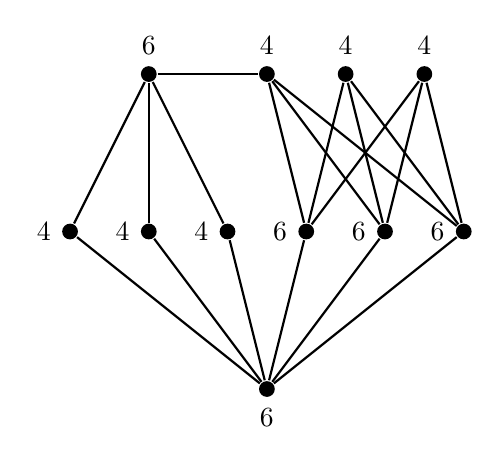
\begin{tikzpicture}[
       thick,
       acteur/.style={
         circle,
         fill=black,
         thick,
         inner sep=2pt,
         minimum size=0.2cm
       }
     ]

       \node (v) at (-3.5,0) [acteur,label=below:$6$]{};
       \node (w1) at (-6,2) [acteur,label=left:$4$]{}; 
       \node (w2) at (-5,2) [acteur,label=left:$4$]{}; 
       \node (w3) at (-4,2) [acteur,label=left:$4$]{};
       \node (w4) at (-3,2) [acteur,label=left:$6$]{};
       \node (w5) at (-2,2) [acteur,label=left:$6$]{};
       \node (w6) at (-1,2) [acteur,label=left:$6$]{};
       
       \node (u1) at (-3.5,4) [acteur,label=above:$4$]{};
  	   \node (u2) at (-2.5,4) [acteur,label=above:$4$]{};
  	   \node (u3) at (-1.5,4) [acteur,label=above:$4$]{};

  	   \node (vs) at (-5,4) [acteur,label=above:$6$]{};
  	   
       \draw (v) -- (w1);
       \draw (v) -- (w2);
       \draw (v) -- (w3);
       \draw (v) -- (w4);
       \draw (v) -- (w5);
       \draw (v) -- (w6);
       
       \draw (w4) -- (u1);
       \draw (w4) -- (u2);
       \draw (w4) -- (u3);
       \draw (w5) -- (u1);
       \draw (w5) -- (u2);
       \draw (w5) -- (u3);
       \draw (w6) -- (u1);
       \draw (w6) -- (u2);
       \draw (w6) -- (u3);
       
       \draw (w1) -- (vs);
       \draw (w2) -- (vs);
       \draw (w3) -- (vs);
       
	   \draw (vs) -- (u1);

\end{tikzpicture}
  \caption{The case $f=6$, $t(G)=0$}
  \label{figure11:Figure 11}
\end{figure}


The case \(t(G)=1\) is almost similar to the preceding case, so let \(v\in [16]\), such that \(\deg_G(v)=6\) and \(|\{w\in A_v:\deg_G(w)=4\}|=3\). According to Lemma \ref{lemma364} such a \(v\) must still exist, since we only have one triangle in \(G\). Again let \(U=\{u_1,u_2,u_3\}\), such that \(\deg_G(u_i)=4\) and \(U\cap A_v=\emptyset\). Then by Lemma \ref{lemma364} again there exists a \(u\in U\) such that \(u\) is adjacent to every \(w\in A_v\) which satisfies \(\deg_G(w)=6\), since at most one of the \(w\in A_v\) which satisfy \(\deg_G(w)=6\) can be contained in a triangle. Now by Lemma \ref{lemma362} there exists a \(v'\in [16]\setminus (\{v\}\cup A_v\cup U)\), such that \(u\) is adjacent to \(v'\) and \(\deg_G(v')=6\) and the rest of the proof is analogous to the preceding case.

\begin{figure}[H]
\centering
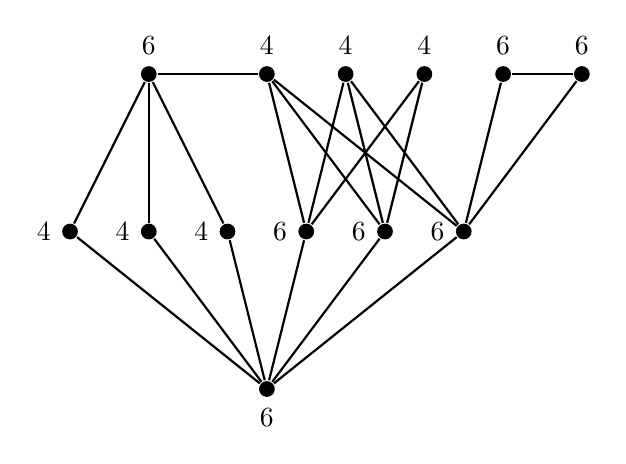
\begin{tikzpicture}[
       thick,
       acteur/.style={
         circle,
         fill=black,
         thick,
         inner sep=2pt,
         minimum size=0.2cm
       }
     ]

       \node (v) at (-3.5,0) [acteur,label=below:$6$]{};
       \node (w1) at (-6,2) [acteur,label=left:$4$]{}; 
       \node (w2) at (-5,2) [acteur,label=left:$4$]{}; 
       \node (w3) at (-4,2) [acteur,label=left:$4$]{};
       \node (w4) at (-3,2) [acteur,label=left:$6$]{};
       \node (w5) at (-2,2) [acteur,label=left:$6$]{};
       \node (w6) at (-1,2) [acteur,label=left:$6$]{};
       
       \node (u1) at (-3.5,4) [acteur,label=above:$4$]{};
  	   \node (u2) at (-2.5,4) [acteur,label=above:$4$]{};
  	   \node (u3) at (-1.5,4) [acteur,label=above:$4$]{};

	   \node (u4) at (-0.5,4) [acteur,label=above:$6$]{};
	   \node (u5) at (0.5,4) [acteur,label=above:$6$]{};
	   
  	   \node (vs) at (-5,4) [acteur,label=above:$6$]{};
  	   
       \draw (v) -- (w1);
       \draw (v) -- (w2);
       \draw (v) -- (w3);
       \draw (v) -- (w4);
       \draw (v) -- (w5);
       \draw (v) -- (w6);
       
       \draw (w4) -- (u1);
       \draw (w4) -- (u2);
       \draw (w4) -- (u3);
       \draw (w5) -- (u1);
       \draw (w5) -- (u2);
       \draw (w5) -- (u3);
       \draw (w6) -- (u1);
       \draw (w6) -- (u2);
       \draw (w6) -- (u4);
       \draw (w6) -- (u5);
       
       \draw (w1) -- (vs);
       \draw (w2) -- (vs);
       \draw (w3) -- (vs);
       
	   \draw (vs) -- (u1);
	   
	   \draw (u4) -- (u5);

\end{tikzpicture}
  \caption{The case $f=6$, $t(G)=1$}
  \label{figure12:Figure 12}
\end{figure}


\end{proof}
\end{thm}